\documentclass[tikz,border=3mm,multi=tikzpicture]{standalone}
\usepackage[utf8]{inputenc}
\usepackage[T1]{fontenc}
\usepackage{helvet}
\renewcommand{\familydefault}{\sfdefault}
\usepackage{tikz}
\usetikzlibrary{arrows.meta,positioning}
\begin{document}

\tikzset{every node/.append style={font=\sffamily\small}}

% TikZ 1
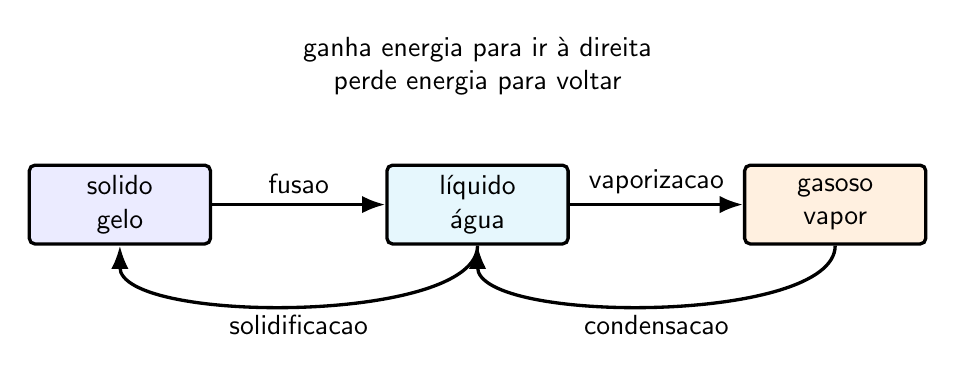
\begin{tikzpicture}[>=Latex,node distance=2.2cm]
  \tikzstyle{state}=[draw,rounded corners=2pt,minimum width=2.3cm,minimum height=1.0cm,align=center,very thick]
  \node[state,fill=blue!8] (s) {solido\\gelo};
  \node[state,fill=cyan!10,right=of s] (l) {líquido\\água};
  \node[state,fill=orange!12,right=of l] (g) {gasoso\\vapor};
  \draw[very thick,->] (s) -- node[above] {fusao} (l);
  \draw[very thick,->] (l) -- node[above] {vaporizacao} (g);
  \draw[very thick,->] (g.south) .. controls +(0,-1.0) and +(0,-1.0) .. node[below] {condensacao} (l.south);
  \draw[very thick,->] (l.south) .. controls +(0,-1.0) and +(0,-1.0) .. node[below] {solidificacao} (s.south);
  \node[align=center,above=0.75cm of l] {ganha energia para ir à direita\\perde energia para voltar};
\end{tikzpicture}

% TikZ 2
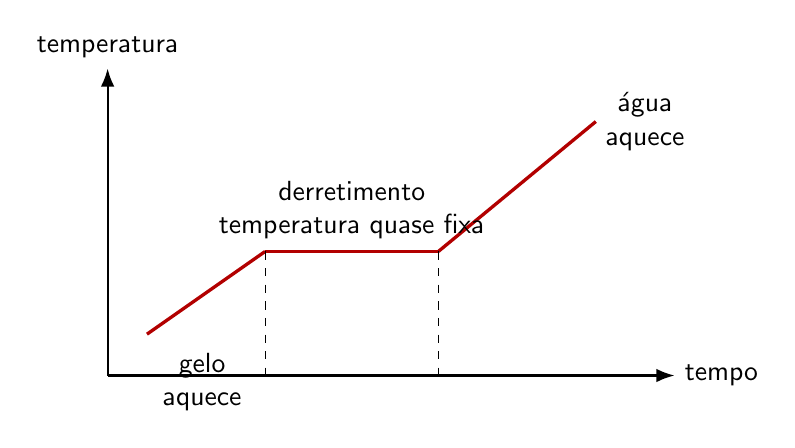
\begin{tikzpicture}[x=1cm,y=0.75cm,>=Latex]
  \draw[->,thick] (0,0) -- (7.2,0) node[right] {tempo};
  \draw[->,thick] (0,0) -- (0,5.2) node[above] {temperatura};
  \draw[very thick,red!70!black] (0.5,0.7) -- (2.0,2.1);
  \draw[very thick,red!70!black] (2.0,2.1) -- (4.2,2.1);
  \draw[very thick,red!70!black] (4.2,2.1) -- (6.2,4.3);
  \node[align=center,below] at (1.2,0.55) {gelo\\aquece};
  \node[align=center,above] at (3.1,2.15) {derretimento\\temperatura quase fixa};
  \node[align=center,right] at (6.2,4.3) {água\\aquece};
  \draw[dashed] (2.0,2.1) -- (2.0,0);
  \draw[dashed] (4.2,2.1) -- (4.2,0);
\end{tikzpicture}

\end{document}
